\documentclass[aspectratio=169, table, 12pt]{beamer}

\usepackage{colortbl}
\usepackage{xcolor}
\usepackage{listings}
\usepackage{tabularx}
\usepackage{tikz}
\usepackage{pgfplots}
\pgfplotsset{compat=1.18}
\usetikzlibrary{arrows.meta, positioning, calc, fit, shapes.geometric}

\makeatletter
\def\input@path{{../theme/}}
\makeatother
\graphicspath{{../theme/}{../../figures/}}
\usetheme{Pradita}

\definecolor{praditagreen}{RGB}{37, 113, 71}

% Tema membuat garis tabel berwarna putih. Dikembalikan agar tabel terbaca.
\arrayrulecolor{black}
\setlength{\arrayrulewidth}{0.5pt}

\lstdefinelanguage{bash}{
  keywords={},
  basicstyle=\ttfamily\scriptsize,
  ndkeywords={curl, k6, grep, cd},
  ndkeywordstyle=\color{purple}\bfseries,
  sensitive=true,
  commentstyle=\color{gray},
  numbers=none,
  breaklines=true,
  frame=lines,
  backgroundcolor=\color{lightgray!10},
  tabsize=2,
  comment=[l]{\#},
  showstringspaces=false
}

\lstdefinelanguage{TypeScript}{
  keywords={const, let, function, return, for, of, new, await, async},
  ndkeywords={console, Promise, setTimeout, number},
  basicstyle=\ttfamily\scriptsize,
  keywordstyle=\color{blue}\bfseries,
  ndkeywordstyle=\color{purple}\bfseries,
  sensitive=true,
  commentstyle=\color{gray}\itshape,
  stringstyle=\color{red},
  numbers=none,
  breaklines=true,
  frame=lines,
  backgroundcolor=\color{lightgray!10},
  tabsize=2,
  comment=[l]{//},
  morestring=[b]",
  showstringspaces=false
}

\lstdefinelanguage{html}{
  basicstyle=\ttfamily\scriptsize,
  keywordstyle=\color{blue}\bfseries,
  stringstyle=\color{red},
  commentstyle=\color{gray}\itshape,
  sensitive=false,
  morecomment=[s]{<!--}{-->},
  morestring=[b]",
  numbers=none,
  breaklines=true,
  frame=lines,
  backgroundcolor=\color{lightgray!10},
  tabsize=2,
  showstringspaces=false
}

\title{\Huge Browser, HTTP, dan\\ \vspace{10pt} Network Internals}
\subtitle{IF140303 - Pengembangan Aplikasi Web}
\author{\textbf{Alfa Yohannis}}

\begin{document}

\frame{\titlepage}

\begin{frame}[fragile]
  \frametitle{Isi Pertemuan}
  \vspace{20pt}
  \begin{columns}[t]
    \column{0.5\textwidth}
    \tableofcontents[sections={1-4}]

    \column{0.5\textwidth}
    \tableofcontents[sections={5-8}]
  \end{columns}
\end{frame}

\begin{frame}{\hfill}
  \centering
  \Huge{\textbf{Mengapa halaman terasa lambat,\\dan di bagian mana?}}
\end{frame}

\section{Tujuan dan Kerangka Bahasan}

\begin{frame}{\hfill}
  \centering
  \Huge{\textbf{Tujuan dan Kerangka Bahasan}}
\end{frame}

\begin{frame}{{\Large Tujuan Pembelajaran}}
  \vspace{15pt}
  \begin{itemize}
    \item Menjelaskan urutan peristiwa sejak alamat diketik sampai halaman
          tampil, beserta biaya waktu tiap tahapnya.
    \item Membedakan HyperText Transfer Protocol (HTTP) versi 1.1, HTTP/2,
          dan HTTP/3 berdasarkan cara ketiganya menangani banyak permintaan
          sekaligus.
    \item Mengukur performa aplikasi web memakai \textit{browser DevTools}
          dan menetapkan angka \textit{baseline} yang dapat diuji ulang.
  \end{itemize}
  \vspace{10pt}
  {\footnotesize Tanpa pengukuran, optimasi tidak bisa akurat.}
\end{frame}

\begin{frame}{{\Large Banyak Sumber Keterlambatan}}
  \vspace{10pt}
  \begin{itemize}
    \item Aplikasi web yang lambat jarang disebabkan oleh satu masalah besar.
    \item Penyebabnya kumpulan keterlambatan kecil yang menumpuk:
    \begin{itemize}
      \item mencari alamat server,
      \item membangun koneksi,
      \item menunggu byte pertama,
      \item mengunduh berkas,
      \item menyusun tampilan.
    \end{itemize}
    \item Tiap tahap punya biaya, dan biaya itu sering tidak terlihat dari
          kode program.
  \end{itemize}
\end{frame}

\section{Arsitektur Browser}

\begin{frame}{\hfill}
  \centering
  \Huge{\textbf{Arsitektur Browser}}
\end{frame}

\begin{frame}{{\Large Bukan Satu Program Tunggal}}
  \vspace{2pt}
  \centering
  \scalebox{0.82}{
  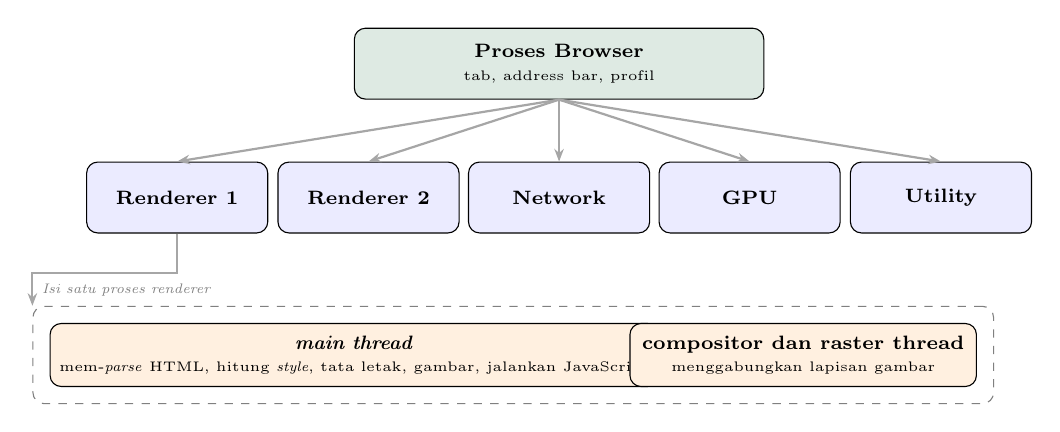
\begin{tikzpicture}[
    font=\scriptsize,
    proses/.style={draw, rounded corners, align=center, minimum height=0.9cm,
                   minimum width=2.3cm, fill=blue!8, font=\scriptsize\bfseries},
    utas/.style={draw, rounded corners, align=center, minimum height=0.8cm,
                 fill=orange!12, font=\scriptsize\bfseries},
    panah/.style={-{Stealth[length=1.6mm]}, gray!70, thick}
  ]
    \node[proses, fill=praditagreen!15, minimum width=5.2cm] (b) at (0,0)
      {Proses Browser\\{\tiny\mdseries tab, address bar, profil}};
    \node[proses] (r1)  at (-4.85,-1.7) {Renderer 1};
    \node[proses] (r2)  at (-2.42,-1.7) {Renderer 2};
    \node[proses] (net) at (0,-1.7)     {Network};
    \node[proses] (gpu) at (2.42,-1.7)  {GPU};
    \node[proses] (ut)  at (4.85,-1.7)  {Utility};
    \foreach \n in {r1,r2,net,gpu,ut} \draw[panah] (b.south) -- (\n.north);

    \node[utas, minimum width=5.6cm] (main) at (-2.6,-3.7)
      {\textit{main thread}\\{\tiny\mdseries mem-\textit{parse} HTML, hitung
       \textit{style}, tata letak, gambar, jalankan JavaScript}};
    \node[utas, minimum width=4.4cm] (comp) at (3.1,-3.7)
      {compositor dan raster thread\\{\tiny\mdseries menggabungkan lapisan gambar}};
    \node[draw, dashed, gray, rounded corners, inner sep=6pt, fit=(main)(comp)] (kotak) {};
    \node[anchor=south west, font=\tiny\itshape, gray] at (kotak.north west) {Isi satu proses renderer};
    \draw[panah] (r1.south) -- ++(0,-0.5) -| (kotak.north west);
  \end{tikzpicture}}

  \vspace{2pt}
  {\footnotesize Satu tab macet tidak mematikan seluruh browser. Situs
  berlainan dipisahkan lewat \textit{site isolation}. Hampir seluruh pekerjaan
  halaman ditanggung satu \textit{main thread}.}
\end{frame}

\begin{frame}{{\Large Tugas Tiap Proses}}
  \vspace{8pt}
  \centering
  {\small
  \begin{tabularx}{0.95\textwidth}{lX}
    \hline
    \textbf{Proses} & \textbf{Tugas} \\
    \hline
    Browser & Mengelola tab, address bar, menu, dan penyimpanan profil. \\
    \hline
    Renderer & Mem-\textit{parse} HTML dan CSS, menjalankan JavaScript, menggambar isi halaman. \\
    \hline
    Network & Menangani DNS, koneksi, dan seluruh lalu lintas HTTP. \\
    \hline
    GPU & Menggabungkan lapisan gambar untuk ditampilkan ke layar. \\
    \hline
    Utility & Menjalankan tugas terpisah seperti pemutaran audio dan video. \\
    \hline
  \end{tabularx}}
\end{frame}

\begin{frame}{{\Large Renderer dan GPU Sering Tertukar}}
  \vspace{10pt}
  \begin{columns}[t]
    \column{0.48\textwidth}
    \textbf{Renderer} menentukan \emph{apa} yang digambar
    \vspace{4pt}
    \begin{itemize}
      \item mem-\textit{parse} HTML dan CSS,
      \item menghitung \textit{style},
      \item menghitung posisi tiap elemen,
      \item menyusun daftar perintah menggambar.
    \end{itemize}

    \column{0.48\textwidth}
    \textbf{GPU} menentukan \emph{bagaimana} perintah itu jadi piksel
    \vspace{4pt}
    \begin{itemize}
      \item menggambar tiap lapisan,
      \item menggabungkan lapisan,
      \item menyerahkan hasilnya ke layar.
    \end{itemize}
  \end{columns}

  \vspace{10pt}
  {\footnotesize Analoginya percetakan: Renderer juru tata letak, GPU mesin
  cetak. Jumlah Renderer bertambah mengikuti situs yang dibuka, sedangkan
  proses GPU cukup satu.}
\end{frame}

\begin{frame}{{\Large Bila Banyak Tab Dibuka}}
  \vspace{5pt}
  \centering
  \scalebox{1.2}{
  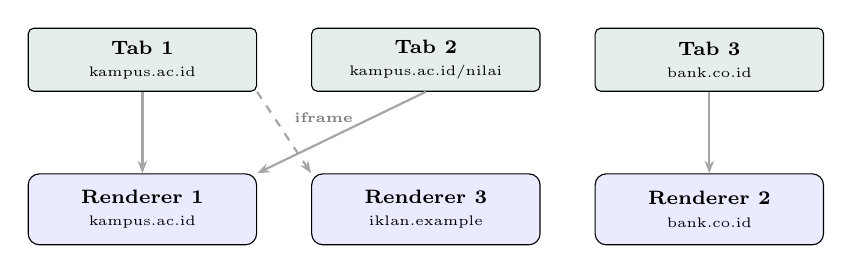
\begin{tikzpicture}[
    font=\scriptsize,
    tab/.style={draw, rounded corners=2pt, align=center, minimum height=0.8cm,
                minimum width=2.9cm, fill=praditagreen!12, font=\scriptsize\bfseries},
    ren/.style={draw, rounded corners, align=center, minimum height=0.9cm,
                minimum width=2.9cm, fill=blue!8, font=\scriptsize\bfseries},
    panah/.style={-{Stealth[length=1.6mm]}, gray!70, thick}
  ]
    \node[tab] (t1) at (-3.6,0) {Tab 1\\{\tiny\mdseries kampus.ac.id}};
    \node[tab] (t2) at (0,0)    {Tab 2\\{\tiny\mdseries kampus.ac.id/nilai}};
    \node[tab] (t3) at (3.6,0)  {Tab 3\\{\tiny\mdseries bank.co.id}};
    \node[ren] (r1) at (-3.6,-1.9) {Renderer 1\\{\tiny\mdseries kampus.ac.id}};
    \node[ren] (r3) at (0,-1.9)    {Renderer 3\\{\tiny\mdseries iklan.example}};
    \node[ren] (r2) at (3.6,-1.9)  {Renderer 2\\{\tiny\mdseries bank.co.id}};
    \draw[panah] (t1.south) -- (r1.north);
    \draw[panah] (t2.south) -- (r1.north east);
    \draw[panah] (t3.south) -- (r2.north);
    \draw[panah, dashed] (t1.south east) -- node[above right, font=\tiny\bfseries, gray] {iframe} (r3.north west);
  \end{tikzpicture}}

  \vspace{6pt}
  {\footnotesize Aturan \textit{process-per-site-instance}: tab situs sama
  berbagi satu \textit{renderer}, situs lain dapat proses sendiri, iframe
  lintas situs dipisahkan.}
\end{frame}

\section{DNS, TCP, dan TLS}

\begin{frame}{\hfill}
  \centering
  \Huge{\textbf{DNS, TCP, dan TLS}}
\end{frame}

\begin{frame}{{\Large Tiga Tahap Sebelum Byte Pertama}}
  \vspace{10pt}
  \centering
  \scalebox{1.2}{
  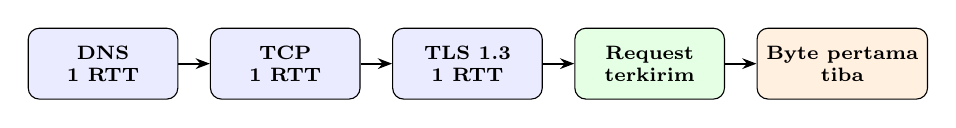
\begin{tikzpicture}[
    node distance=0.45cm and 0.4cm,
    tahap/.style={draw, rounded corners, minimum height=0.9cm, minimum width=1.9cm,
                  align=center, font=\scriptsize\bfseries},
    panah/.style={-{Stealth[length=1.8mm]}, thick}
  ]
    \node[tahap, fill=blue!8]   (dns)  {DNS\\1 RTT};
    \node[tahap, fill=blue!8,  right=of dns]  (tcp)  {TCP\\1 RTT};
    \node[tahap, fill=blue!8,  right=of tcp]  (tls)  {TLS 1.3\\1 RTT};
    \node[tahap, fill=green!10, right=of tls] (req)  {Request\\terkirim};
    \node[tahap, fill=orange!12, right=of req] (ttfb) {Byte pertama\\tiba};
    \draw[panah] (dns) -- (tcp);
    \draw[panah] (tcp) -- (tls);
    \draw[panah] (tls) -- (req);
    \draw[panah] (req) -- (ttfb);
  \end{tikzpicture}}

  \vspace{10pt}
  \begin{itemize}
    \item \textbf{DNS} menerjemahkan nama domain menjadi alamat IP.
    \item \textbf{TCP} membuka koneksi lewat SYN, SYN-ACK, dan ACK.
    \item \textbf{TLS} memeriksa sertifikat lalu menyepakati kunci sesi.
  \end{itemize}
\end{frame}

\begin{frame}{{\Large Jarak yang Menentukan}}
  \vspace{5pt}
  \centering
  {\small
  \begin{tabularx}{0.9\textwidth}{lXrr}
    \hline
    \textbf{Lokasi server} & \textbf{Contoh} & \textbf{RTT} & \textbf{3 RTT} \\
    \hline
    Satu kota  & Jakarta ke Jakarta   & 10 ms  & 30 ms  \\
    \hline
    Regional   & Jakarta ke Singapura & 35 ms  & 105 ms \\
    \hline
    Antarbenua & Jakarta ke Frankfurt & 190 ms & 570 ms \\
    \hline
  \end{tabularx}}

  \vspace{10pt}
  \begin{itemize}
    \item Paket melewati modem, jaringan akses, titik pertukaran trafik,
          kabel darat dan laut, sampai perangkat di pusat data.
    \item Cahaya di serat optik merambat sekitar 200.000 km per detik,
          sehingga Jakarta ke Frankfurt saja butuh sekitar 110 ms.
    \item Angka itu habis sebelum server mengerjakan apa pun.
  \end{itemize}
\end{frame}

\begin{frame}[fragile]{{\Large Mengukur Tiap Tahap Sendiri}}
  \vspace{5pt}
\begin{lstlisting}[language=bash]
curl -o /dev/null -s -w @format-curl.txt https://www.pradita.ac.id/

# dns:0.009726s tcp:0.033991s tls:0.084639s
# ttfb:0.338771s total:0.342899s versi:HTTP/2
\end{lstlisting}

  \vspace{5pt}
  \begin{itemize}
    \item Angka \texttt{curl} bersifat kumulatif, jadi durasi tiap tahap
          diperoleh dengan pengurangan.
    \item Cara menekan biayanya: pakai ulang koneksi, pasang
          \texttt{preconnect}, pilih TLS 1.3, batasi jumlah domain.
    \item CDN menempatkan salinan aset di \textit{edge server} terdekat,
          sehingga jarak ke \textit{origin} tidak lagi dibayar tiap permintaan.
  \end{itemize}
\end{frame}

\section{HTTP/1.1, HTTP/2, dan HTTP/3}

\begin{frame}{\hfill}
  \centering
  \Huge{\textbf{HTTP/1.1, HTTP/2, dan HTTP/3}}
\end{frame}

\begin{frame}{{\Large HTTP/1.1: Satu per Koneksi}}
  \vspace{5pt}
  \centering
  \scalebox{1.35}{
  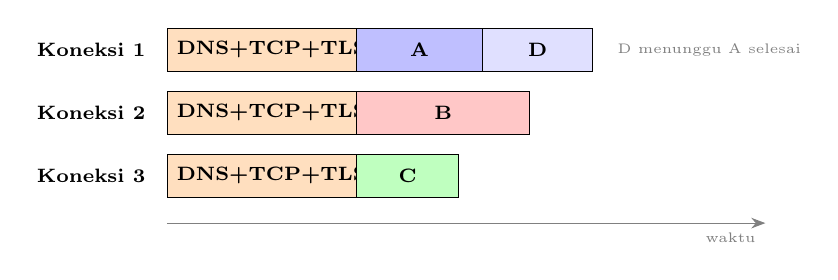
\begin{tikzpicture}[
    font=\scriptsize,
    blok/.style={draw, minimum height=0.55cm, anchor=west, align=center,
                 font=\scriptsize\bfseries},
    setup/.style={blok, fill=orange!25, minimum width=2.4cm},
    baris/.style={anchor=east, font=\scriptsize\bfseries}
  ]
    \node[baris] at (-0.15,0)    {Koneksi 1};
    \node[baris] at (-0.15,-0.8) {Koneksi 2};
    \node[baris] at (-0.15,-1.6) {Koneksi 3};
    \node[setup] at (0,0)    {DNS+TCP+TLS};
    \node[setup] at (0,-0.8) {DNS+TCP+TLS};
    \node[setup] at (0,-1.6) {DNS+TCP+TLS};
    \node[blok, minimum width=1.6cm, fill=blue!25]  at (2.4,0)    {A};
    \node[blok, minimum width=1.4cm, fill=blue!12]  at (4.0,0)    {D};
    \node[blok, minimum width=2.2cm, fill=red!22]   at (2.4,-0.8) {B};
    \node[blok, minimum width=1.3cm, fill=green!25] at (2.4,-1.6) {C};
    \node[anchor=west, font=\tiny, gray] at (5.6,0) {D menunggu A selesai};
    \draw[-{Stealth[length=1.8mm]}, gray] (0,-2.2) -- (7.6,-2.2)
      node[anchor=north east, font=\tiny] {waktu};
  \end{tikzpicture}}

  \vspace{6pt}
  {\footnotesize Gejalanya disebut \textit{head-of-line blocking}. Browser
  menyiasatinya dengan membuka sekitar enam koneksi paralel per domain, dan
  tiap koneksi menanggung biaya pembukaan sendiri.}
\end{frame}

\begin{frame}{{\Large HTTP/2: Berbagi Satu Koneksi}}
  \vspace{5pt}
  \centering
  \scalebox{1.35}{
  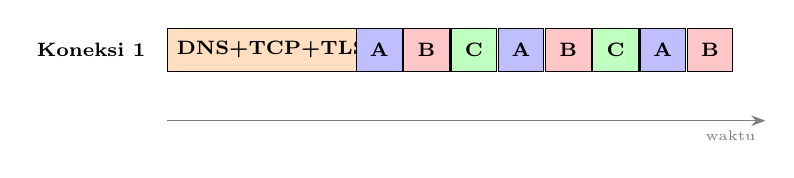
\begin{tikzpicture}[
    font=\scriptsize,
    blok/.style={draw, minimum height=0.55cm, anchor=west, align=center,
                 font=\scriptsize\bfseries},
    setup/.style={blok, fill=orange!25, minimum width=2.4cm},
    baris/.style={anchor=east, font=\scriptsize\bfseries}
  ]
    \node[baris] at (-0.15,0) {Koneksi 1};
    \node[setup] at (0,0) {DNS+TCP+TLS};
    \foreach \i/\w/\t in {0/blue!25/A, 1/red!22/B, 2/green!25/C, 3/blue!25/A,
                          4/red!22/B, 5/green!25/C, 6/blue!25/A, 7/red!22/B} {
      \pgfmathsetmacro{\x}{2.4 + \i*0.6}
      \node[blok, minimum width=0.58cm, fill=\w] at (\x,0) {\t};
    }
    \draw[-{Stealth[length=1.8mm]}, gray] (0,-0.9) -- (7.6,-0.9)
      node[anchor=north east, font=\tiny] {waktu};
  \end{tikzpicture}}

  \vspace{8pt}
  \begin{itemize}
    \item Data dipecah menjadi \textit{frame} biner, lalu diselang-seling
          dalam satu koneksi. Cara ini disebut \textit{multiplexing}.
    \item Header di-\textit{compress} memakai HPACK lewat tabel statis dan dinamis.
    \item Sisa masalahnya: satu paket hilang menahan seluruh koneksi TCP.
  \end{itemize}
\end{frame}

\begin{frame}{{\Large HTTP/3: Aliran yang Saling Bebas}}
  \vspace{5pt}
  \centering
  \scalebox{1.35}{
  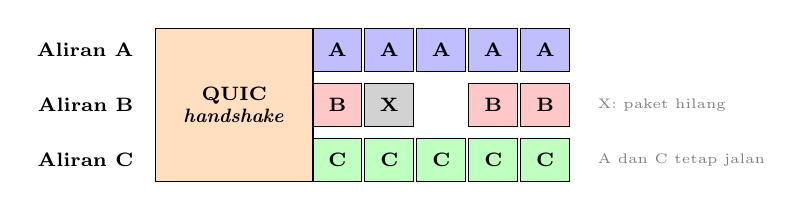
\begin{tikzpicture}[
    font=\scriptsize,
    blok/.style={draw, minimum height=0.55cm, anchor=west, align=center,
                 font=\scriptsize\bfseries},
    setup/.style={blok, fill=orange!25, minimum width=2.0cm},
    baris/.style={anchor=east, font=\scriptsize\bfseries}
  ]
    \node[baris] at (-0.15,0)    {Aliran A};
    \node[baris] at (-0.15,-0.7) {Aliran B};
    \node[baris] at (-0.15,-1.4) {Aliran C};
    \node[setup, minimum height=1.95cm, align=center] at (0,-0.7) {QUIC\\\textit{handshake}};
    \foreach \i in {0,1,2,3,4} {
      \pgfmathsetmacro{\x}{2.0 + \i*0.66}
      \node[blok, minimum width=0.62cm, fill=blue!25]  at (\x,0)    {A};
      \node[blok, minimum width=0.62cm, fill=green!25] at (\x,-1.4) {C};
    }
    \node[blok, minimum width=0.62cm, fill=red!22]  at (2.0,-0.7)  {B};
    \node[blok, minimum width=0.62cm, fill=gray!35] at (2.66,-0.7) {X};
    \node[blok, minimum width=0.62cm, fill=red!22]  at (3.98,-0.7) {B};
    \node[blok, minimum width=0.62cm, fill=red!22]  at (4.64,-0.7) {B};
    \node[anchor=west, font=\tiny, gray] at (5.5,-0.7) {X: paket hilang};
    \node[anchor=west, font=\tiny, gray] at (5.5,-1.4) {A dan C tetap jalan};
  \end{tikzpicture}}

  \vspace{6pt}
  {\footnotesize QUIC memindahkan pencatatan urutan dari tingkat koneksi ke
  tingkat aliran, menyatukan \textit{handshake} sehingga cukup satu RTT, dan
  mengenali koneksi lewat \textit{connection ID} sehingga tahan perpindahan
  jaringan.}
\end{frame}

\begin{frame}{{\Large Ringkasan Perbedaan Tiga Versi}}
  \vspace{5pt}
  \centering
  {\small
  \begin{tabularx}{\textwidth}{lXXX}
    \hline
     & \textbf{HTTP/1.1} & \textbf{HTTP/2} & \textbf{HTTP/3} \\
    \hline
    Format & Teks & Biner & Biner \\
    \hline
    Transport & TCP & TCP & QUIC di atas UDP \\
    \hline
    Permintaan sekaligus & Satu per koneksi & Banyak, diselang-seling & Banyak, aliran mandiri \\
    \hline
    Blocking & Di tingkat permintaan & Di tingkat TCP & Hanya aliran terdampak \\
    \hline
    Header & Dikirim penuh & Di-\textit{compress} HPACK & Di-\textit{compress} QPACK \\
    \hline
    Pindah jaringan & Koneksi putus & Koneksi putus & Berlanjut lewat \textit{connection ID} \\
    \hline
  \end{tabularx}}

  \vspace{8pt}
  {\footnotesize Jumlah aset tetap penting pada ketiga versi, karena tiap aset
  menuntut permintaan, \textit{parsing}, dan pemakaian memori.}
\end{frame}

\section{Siklus Hidup Request dan Event Loop}

\begin{frame}{\hfill}
  \centering
  \Huge{\textbf{Siklus Hidup Request\\dan Event Loop}}
\end{frame}

\begin{frame}{{\Large Satu Putaran Event Loop}}
  \vspace{8pt}
  \centering
  \scalebox{1.2}{
  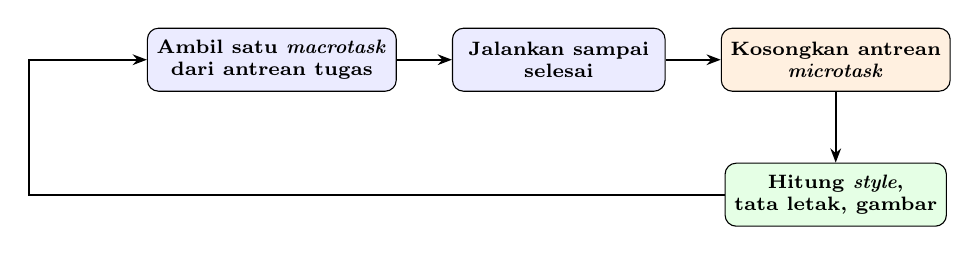
\begin{tikzpicture}[
    node distance=0.5cm and 0.7cm,
    kotak/.style={draw, rounded corners, minimum height=0.8cm, minimum width=2.7cm,
                  align=center, font=\scriptsize\bfseries},
    panah/.style={-{Stealth[length=1.8mm]}, thick}
  ]
    \node[kotak, fill=blue!8] (task) {Ambil satu \textit{macrotask}\\dari antrean tugas};
    \node[kotak, fill=blue!8, right=of task] (jalan) {Jalankan sampai\\selesai};
    \node[kotak, fill=orange!12, right=of jalan] (micro) {Kosongkan antrean\\\textit{microtask}};
    \node[kotak, fill=green!10, below=0.9cm of micro] (render) {Hitung \textit{style},\\tata letak, gambar};
    \draw[panah] (task) -- (jalan);
    \draw[panah] (jalan) -- (micro);
    \draw[panah] (micro) -- (render);
    \draw[panah] (render) -| ([xshift=-1.5cm]task.west) -- (task.west);
  \end{tikzpicture}}

  \vspace{8pt}
  {\footnotesize Penggambaran layar bukan proses terpisah, melainkan salah
  satu tahap dalam putaran yang sama, dan berbagi \textit{main thread} dengan
  JavaScript.}
\end{frame}

\begin{frame}{{\Large Dua Antrean, Dua Perlakuan}}
  \vspace{5pt}
  \centering
  {\small
  \begin{tabularx}{\textwidth}{lXX}
    \hline
     & \textbf{\textit{Task queue} (\textit{macrotask})} & \textbf{Antrean \textit{microtask}} \\
    \hline
    Jumlah antrean & Boleh lebih dari satu, dipisah per sumber & Hanya satu \\
    \hline
    Diambil tiap putaran & Satu tugas saja & Dikosongkan seluruhnya \\
    \hline
    Pekerjaan baru saat berjalan & Menunggu putaran berikutnya & Ikut dikerjakan pada putaran yang sama \\
    \hline
    Penggambaran layar & Boleh terjadi sesudahnya & Ditahan sampai antrean kosong \\
    \hline
  \end{tabularx}}
\end{frame}

\begin{frame}[fragile]{{\Large Urutan Eksekusi dan Long Task}}
  \vspace{3pt}
\begin{lstlisting}[language=TypeScript]
console.log("1: kode sinkron");
setTimeout(() => console.log("4: macrotask berikutnya"), 0);
Promise.resolve().then(() => console.log("3: microtask"));
console.log("2: kode sinkron");
// Keluaran berurutan: 1, 2, 3, 4
\end{lstlisting}

  \vspace{3pt}
  \begin{itemize}
    \item Tugas berjalan sampai selesai tanpa dapat dipotong, sehingga tugas
          lebih dari 50 milidetik disebut \textit{long task}.
    \item Selama tugas berjalan, tidak ada penggambaran ulang dan tidak ada
          tanggapan atas klik.
    \item Dua jalan keluar: pecah pekerjaan menjadi potongan kecil, atau
          pindahkan ke \textit{web worker}.
  \end{itemize}
\end{frame}

\section{Rendering Pipeline}

\begin{frame}{\hfill}
  \centering
  \Huge{\textbf{Rendering Pipeline dan\\Critical Rendering Path}}
\end{frame}

\begin{frame}{{\Large Dari Berkas Mentah sampai Piksel}}
  \vspace{10pt}
  \centering
  \scalebox{1.2}{
  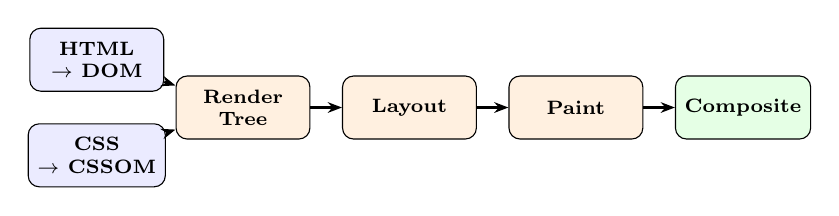
\begin{tikzpicture}[
    node distance=0.4cm and 0.4cm,
    tahap/.style={draw, rounded corners, minimum height=0.8cm, minimum width=1.7cm,
                  align=center, font=\scriptsize\bfseries},
    panah/.style={-{Stealth[length=1.8mm]}, thick}
  ]
    \node[tahap, fill=blue!8] (html) {HTML\\$\rightarrow$ DOM};
    \node[tahap, fill=blue!8, below=of html] (css) {CSS\\$\rightarrow$ CSSOM};
    \node[tahap, fill=orange!12, right=1cm of $(html)!0.5!(css)$] (tree) {Render\\Tree};
    \node[tahap, fill=orange!12, right=of tree] (layout) {Layout};
    \node[tahap, fill=orange!12, right=of layout] (paint) {Paint};
    \node[tahap, fill=green!10, right=of paint] (comp) {Composite};
    \draw[panah] (html) -- (tree);
    \draw[panah] (css) -- (tree);
    \draw[panah] (tree) -- (layout);
    \draw[panah] (layout) -- (paint);
    \draw[panah] (paint) -- (comp);
  \end{tikzpicture}}

  \vspace{10pt}
  {\footnotesize Analoginya penyusunan koran: DOM naskah yang sudah diketik,
  CSSOM panduan \textit{style}, Layout penentuan posisi, Paint penggambaran
  isi, Composite penggabungan lapisan.}
\end{frame}

\begin{frame}[fragile]{{\Large Dua Penghambat yang Paling Sering Muncul}}
  \vspace{3pt}
  \begin{itemize}
    \item \textbf{CSS bersifat \textit{render blocking}}: halaman tidak
          digambar sebelum seluruh CSS diunduh dan di-\textit{parse}.
    \item \textbf{Script tanpa penanda bersifat \textit{parser blocking}}:
          penguraian HTML berhenti sampai berkas selesai dijalankan.
  \end{itemize}
  \vspace{3pt}
\begin{lstlisting}[language=html]
<!-- Menahan parsing HTML sampai selesai dijalankan -->
<script src="/js/analytics.js"></script>

<!-- Paralel dengan parsing, jalan setelah parsing selesai, urut -->
<script src="/js/aplikasi.js" defer></script>

<!-- Paralel juga, langsung jalan begitu unduhan selesai, tidak urut -->
<script src="/js/iklan.js" async></script>
\end{lstlisting}
\end{frame}

\section{Core Web Vitals}

\begin{frame}{\hfill}
  \centering
  \Huge{\textbf{Core Web Vitals}}
\end{frame}

\begin{frame}{{\Large Tiga Angka Inti}}
  \vspace{5pt}
  \centering
  {\small
  \begin{tabularx}{0.95\textwidth}{lXll}
    \hline
    \textbf{Metrik} & \textbf{Pertanyaan pengguna} & \textbf{Baik} & \textbf{Buruk} \\
    \hline
    LCP & Kapan isi utama terlihat?          & $\leq$ 2,5 detik & $>$ 4 detik \\
    \hline
    INP & Seberapa cepat halaman menanggapi? & $\leq$ 200 ms    & $>$ 500 ms \\
    \hline
    CLS & Apakah tata letak melompat?        & $\leq$ 0,1       & $>$ 0,25 \\
    \hline
  \end{tabularx}}

  \vspace{10pt}
  \begin{itemize}
    \item LCP diukur dalam waktu, begitu pula INP. CLS tidak bersatuan,
          karena berupa skor perkalian dua pecahan.
    \item INP hanya menghitung klik, ketukan, dan penekanan tombol.
          \textit{Scroll} dan \textit{hover} tidak dihitung.
  \end{itemize}
\end{frame}

\begin{frame}{{\Large Tiga Bagian Penyusun Jeda INP}}
  \vspace{5pt}
  \centering
  {\small
  \begin{tabularx}{0.95\textwidth}{lX}
    \hline
    \textbf{Bagian} & \textbf{Isinya} \\
    \hline
    \textit{Input delay} & Menunggu \textit{main thread} bebas dari tugas yang sedang berjalan \\
    \hline
    \textit{Processing time} & Menjalankan \textit{event handler} milik aplikasi \\
    \hline
    \textit{Presentation delay} & Menghitung \textit{style} dan tata letak, menggambar, sampai \textit{frame} baru tampil \\
    \hline
  \end{tabularx}}

  \vspace{8pt}
  {\footnotesize Tombol yang ditekan saat ada tugas 300 milidetik berjalan
  sudah kalah sejak bagian pertama, walaupun isi \textit{handler}-nya hanya
  satu baris.}
\end{frame}

\begin{frame}{{\Large Persentil ke-75, Bukan Rata-rata}}
  \vspace{10pt}
  \begin{itemize}
    \item Seluruh kunjungan diurutkan dari tercepat sampai terlambat, lalu
          diambil nilai pada urutan 75 persen.
    \item Artinya 75 persen kunjungan sama cepat atau lebih cepat, sedangkan
          25 persen sisanya lebih lambat.
    \item Rata-rata menyesatkan: 90 kunjungan dengan LCP 1 detik menutupi 10
          kunjungan dengan LCP 8 detik, dan rata-ratanya tetap terlihat bagus
          di 1,7 detik.
    \item Pengukuran di komputer pengembang disebut \textit{lab data}, dan
          hasilnya hampir selalu lebih baik daripada kenyataan.
  \end{itemize}
\end{frame}

\section{Praktik: DevTools}

\begin{frame}{\hfill}
  \centering
  \Huge{\textbf{Praktik: DevTools}}
\end{frame}

\begin{frame}{{\Large Empat Panel yang Dipakai}}
  \vspace{8pt}
  \centering
  {\small
  \begin{tabularx}{0.95\textwidth}{lX}
    \hline
    \textbf{Panel} & \textbf{Kegunaan} \\
    \hline
    Network & Melihat urutan permintaan, ukuran berkas, dan rincian waktu tiap tahap. \\
    \hline
    Performance & Melihat pekerjaan \textit{main thread} dan menemukan \textit{long task}. \\
    \hline
    Lighthouse & Menjalankan audit performa dan aksesibilitas secara otomatis. \\
    \hline
    Coverage & Menghitung berapa persen CSS dan JavaScript yang benar-benar terpakai. \\
    \hline
  \end{tabularx}}
\end{frame}

\begin{frame}{{\Large Panel Network}}
  \vspace{2pt}
  \centering
  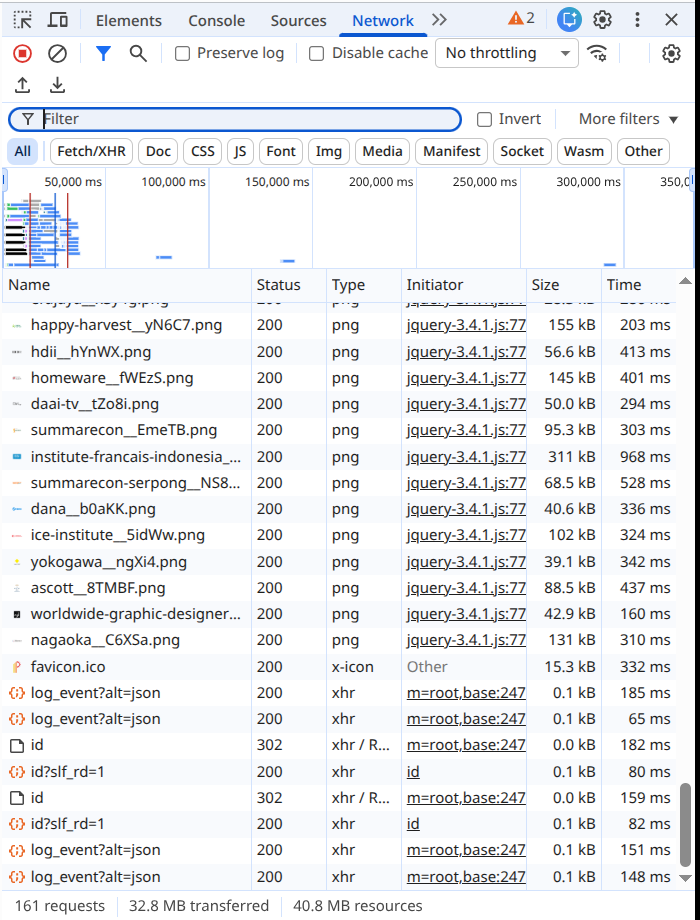
\includegraphics[width=0.52\textwidth, height=0.66\textheight, keepaspectratio]{devtools-network.png}

  \vspace{2pt}
  {\footnotesize Centang \emph{Disable cache} dan \emph{Preserve log} sebelum
  memuat ulang halaman.}
\end{frame}

\begin{frame}{{\Large Menambahkan Dua Kolom Penting}}
  \vspace{2pt}
  \centering
  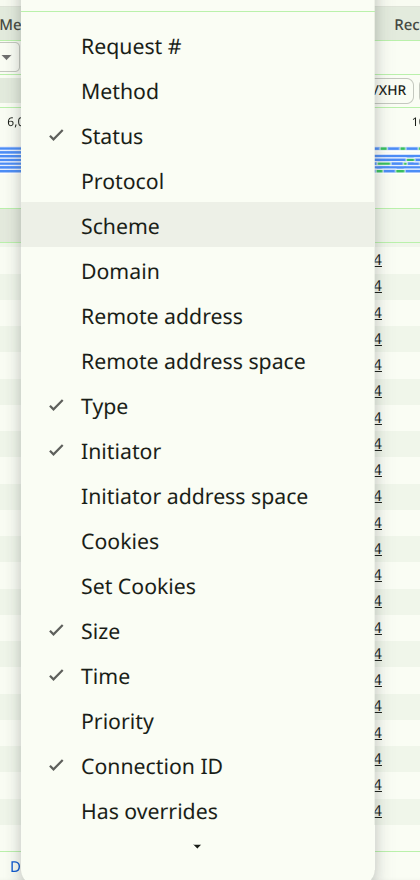
\includegraphics[width=0.28\textwidth, height=0.66\textheight, keepaspectratio]{devtools-menu-kolom-crop.png}

  \vspace{2pt}
  {\footnotesize Klik kanan tepat pada baris judul tabel permintaan. Menu
  tertutup tiap kali satu butir dipilih, sehingga dua kolom menuntut dua kali
  klik kanan.}
\end{frame}

\begin{frame}{{\Large Membaca Kolom Connection ID}}
  \vspace{2pt}
  \centering
  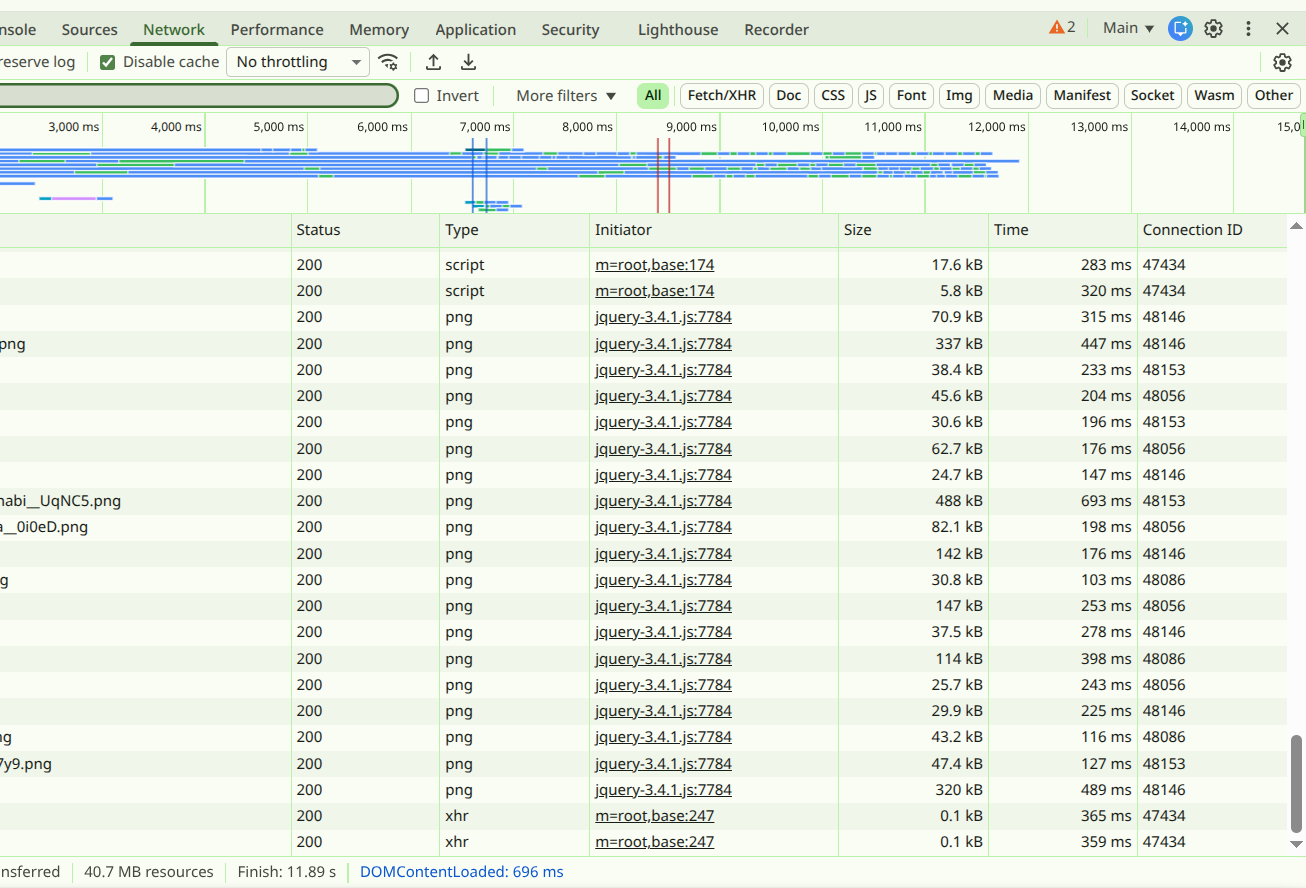
\includegraphics[width=0.72\textwidth, height=0.62\textheight, keepaspectratio]{devtools-kolom-koneksi.png}

  \vspace{2pt}
  {\footnotesize Nomor yang sama berarti permintaan berbagi satu koneksi.
  Nomor berbeda berarti koneksi terpisah.}
\end{frame}

\begin{frame}{{\Large Siapa Mengerjakan Tiap Tahap}}
  \vspace{5pt}
  \centering
  {\small
  \begin{tabularx}{0.97\textwidth}{Xl}
    \hline
    \textbf{Tahap} & \textbf{Penanggung jawab} \\
    \hline
    Menghitung \textit{style}, tata letak, merekam perintah gambar & Renderer, \textit{main thread} \\
    \hline
    Membagi lapisan, menangani \textit{scroll} dan \texttt{transform} & Renderer, \textit{compositor} \\
    \hline
    Mengubah perintah gambar menjadi piksel & Renderer, \textit{raster thread} \\
    \hline
    Menggabungkan lapisan lalu menampilkannya & Proses GPU \\
    \hline
    Menggambar antarmuka browser & Proses Browser \\
    \hline
  \end{tabularx}}
\end{frame}

\section{Latihan 1: Baseline Performa}

\begin{frame}{\hfill}
  \centering
  \Huge{\textbf{Latihan 1\\Baseline Performa}}
\end{frame}

\begin{frame}{{\Large Langkah Kerja}}
  \vspace{5pt}
  \begin{enumerate}
    \item Buka \texttt{www.pradita.ac.id} pada jendela penyamaran.
    \item Aktifkan Slow 4G dan pembatasan CPU empat kali lebih lambat, lalu
          muat ulang dengan \textit{cache} dikosongkan.
    \item Catat rincian waktu lima permintaan terlambat pada panel Network.
    \item Rekam panel Performance, catat seluruh \textit{long task}.
    \item Jalankan Lighthouse mode Mobile, catat LCP, INP, dan CLS.
    \item Ukur TTFB memakai \texttt{ukur-koneksi.sh}, 20 kali, ambil p50 dan p95.
    \item Ulangi pada \texttt{www.pradita.ac.id/praktisi-akademisi}.
  \end{enumerate}
  \vspace{4pt}
  {\footnotesize Pengukuran bersifat mengamati, bukan membebani. Uji beban
  hanya untuk sistem sendiri atau yang sudah berizin.}
\end{frame}

\begin{frame}{{\Large Lembar Isian Baseline}}
  \vspace{5pt}
  \centering
  {\small
  \begin{tabularx}{0.97\textwidth}{lXcc}
    \hline
    \textbf{Metrik} & \textbf{Cara pengukuran} & \textbf{Depan} & \textbf{Praktisi} \\
    \hline
    LCP & Lighthouse, mode Mobile & \dots & \dots \\
    \hline
    INP & Lighthouse, mode Mobile & \dots & \dots \\
    \hline
    CLS & Lighthouse, mode Mobile & \dots & \dots \\
    \hline
    TTFB p50 & \texttt{curl}, 20 permintaan & \dots & \dots \\
    \hline
    TTFB p95 & \texttt{curl}, 20 permintaan & \dots & \dots \\
    \hline
    Jumlah aset & Panel Network & \dots & \dots \\
    \hline
    Total byte & Panel Network & \dots & \dots \\
    \hline
    \textit{Long task} & Panel Performance & \dots & \dots \\
    \hline
  \end{tabularx}}
\end{frame}

\section{Latihan 2: Biaya Koneksi}

\begin{frame}{\hfill}
  \centering
  \Huge{\textbf{Latihan 2\\Biaya Pembukaan Koneksi}}
\end{frame}

\begin{frame}[fragile]{{\Large Menjalankan Pengukuran}}
  \vspace{3pt}
\begin{lstlisting}[language=bash]
cd sources/chapter02
./ukur-koneksi.sh https://www.pradita.ac.id/ 5
\end{lstlisting}

  \vspace{3pt}
  \begin{itemize}
    \item Ulangi untuk tiga domain: kampus, kampus negara tetangga, dan
          kampus di benua lain.
    \item Ambil nilai tengah dari lima pengukuran.
    \item Jawab: berapa persen waktu habis sebelum byte pertama, tahap mana
          yang terbesar, dan apakah yang terjauh selalu paling lambat.
  \end{itemize}
\end{frame}

\begin{frame}{{\Large Arti Tiap Tahap}}
  \vspace{5pt}
  \centering
  {\small
  \begin{tabularx}{0.97\textwidth}{lXX}
    \hline
    \textbf{Tahap} & \textbf{Yang diukur} & \textbf{Rumus} \\
    \hline
    DNS & Lama mencari alamat IP & \texttt{namelookup} \\
    \hline
    TCP & Lama membangun koneksi & \texttt{connect} kurangi \texttt{namelookup} \\
    \hline
    TLS & Lama memeriksa sertifikat dan menyepakati kunci & \texttt{appconnect} kurangi \texttt{connect} \\
    \hline
    Tunggu server & Lama server memproses sampai byte pertama & \texttt{starttransfer} kurangi \texttt{appconnect} \\
    \hline
    Unduh isi & Lama memindahkan sisa isi respons & \texttt{total} kurangi \texttt{starttransfer} \\
    \hline
  \end{tabularx}}
\end{frame}

\begin{frame}{{\Large Contoh Hasil dan Lembar Isian}}
  \vspace{3pt}
  \centering
  {\small \textbf{Contoh terisi, dalam milidetik}\\[3pt]
  \begin{tabularx}{0.9\textwidth}{Xccccc}
    \hline
    \textbf{Domain} & \textbf{DNS} & \textbf{TCP} & \textbf{TLS} & \textbf{Tunggu} & \textbf{Total} \\
    \hline
    \texttt{www.pradita.ac.id} & 9 & 46 & 52 & 78 & 188 \\
    \hline
    \texttt{nus.edu.sg} & 9 & 47 & 62 & 36 & 155 \\
    \hline
    \texttt{ethz.ch} & 1 & 39 & 395 & 421 & 855 \\
    \hline
  \end{tabularx}}

  \vspace{6pt}
  {\small \textbf{Lembar isian}\\[3pt]
  \begin{tabularx}{0.9\textwidth}{Xccccc}
    \hline
    \textbf{Domain} & \textbf{DNS} & \textbf{TCP} & \textbf{TLS} & \textbf{Tunggu} & \textbf{Total} \\
    \hline
    \texttt{www.pradita.ac.id} & \dots & \dots & \dots & \dots & \dots \\
    \hline
    Regional: \dots & \dots & \dots & \dots & \dots & \dots \\
    \hline
    Antarbenua: \dots & \dots & \dots & \dots & \dots & \dots \\
    \hline
  \end{tabularx}}
\end{frame}

\begin{frame}{{\Large Kejanggalan yang Sengaja Dibiarkan}}
  \vspace{10pt}
  \begin{itemize}
    \item Domain terjauh memang paling lambat, tetapi tahap TCP ketiganya
          justru mirip.
    \item Penyebabnya, ketiga situs berada di belakang CDN, sehingga koneksi
          berhenti di \textit{edge server} terdekat.
    \item Sisa perjalanan menuju \textit{origin} baru terasa pada tahap TLS
          dan tunggu server.
    \item Hasil tiap mahasiswa akan berbeda, karena bergantung lokasi
          pengukur dan waktu pengukuran.
  \end{itemize}
\end{frame}

\section{Latihan 3: HTTP/1.1 dan HTTP/2}

\begin{frame}{\hfill}
  \centering
  \Huge{\textbf{Latihan 3\\HTTP/1.1 dan HTTP/2}}
\end{frame}

\begin{frame}[fragile]{{\Large Menjalankan Perbandingan}}
  \vspace{3pt}
\begin{lstlisting}[language=bash]
cd sources/chapter02
./banding-http.sh https://www.pradita.ac.id/ 5
\end{lstlisting}

  \vspace{3pt}
  \begin{itemize}
    \item Skrip mengumpulkan lima aset milik host itu sendiri, memeriksa
          versi HTTP tiap host, lalu menjalankan empat skenario.
    \item Pada browser, konkurensi tidak dapat ditentukan sendiri, sehingga
          baris browser diisi dari pengamatan, bukan dari skenario.
    \item Nama aset dibaca dari \texttt{aset.txt}, lalu diketik satu per satu
          pada kotak filter panel Network.
  \end{itemize}
\end{frame}

\begin{frame}{{\Large Contoh Hasil Empat Skenario}}
  \vspace{5pt}
  \centering
  {\small
  \begin{tabularx}{0.97\textwidth}{Xcccc}
    \hline
    \textbf{Skenario} & \textbf{Aset} & \textbf{Konkurensi} & \textbf{Koneksi} & \textbf{Waktu} \\
    \hline
    HTTP/1.1 berurutan, koneksi baru & 5 & 1 & 5 & 2,14 detik \\
    \hline
    HTTP/1.1 berurutan, dipakai ulang & 5 & 1 & 1 & 1,66 detik \\
    \hline
    HTTP/1.1 serentak & 5 & 5 & 5 & 1,92 detik \\
    \hline
    HTTP/2 serentak & 5 & 5 & 1 & 0,63 detik \\
    \hline
  \end{tabularx}}

  \vspace{6pt}
  {\footnotesize Dua baris pertama sama-sama berurutan, jadi lima koneksinya
  dibuka bergantian, bukan bersamaan. Dua baris terakhir barulah paralel.}
\end{frame}

\begin{frame}{{\Large Lembar Isian Latihan 3}}
  \vspace{5pt}
  \centering
  {\small
  \begin{tabularx}{0.97\textwidth}{Xcccc}
    \hline
    \textbf{Skenario} & \textbf{Aset} & \textbf{Konkurensi} & \textbf{Koneksi} & \textbf{Waktu} \\
    \hline
    Browser, dari kolom \emph{Connection ID} & 5 & \dots & \dots & \dots \\
    \hline
    HTTP/1.1 berurutan, koneksi baru & 5 & 1 & \dots & \dots \\
    \hline
    HTTP/1.1 berurutan, dipakai ulang & 5 & 1 & \dots & \dots \\
    \hline
    HTTP/1.1 serentak & 5 & 5 & \dots & \dots \\
    \hline
    HTTP/2 serentak & 5 & 5 & \dots & \dots \\
    \hline
  \end{tabularx}}

  \vspace{6pt}
  {\footnotesize Pertanyaan: mengapa skenario pertama memakai lima koneksi
  tetapi tetap paling lambat, dan apa beda skenario ketiga dengan keempat?}
\end{frame}

\section{Ringkasan}

\begin{frame}{\hfill}
  \centering
  \Huge{\textbf{Ringkasan}}
\end{frame}

\begin{frame}{{\Large Ringkasan}}
  \vspace{10pt}
  \begin{itemize}
    \item Browser berjalan sebagai banyak proses, tetapi hampir seluruh
          pekerjaan satu halaman ditanggung satu \textit{main thread}.
    \item DNS, TCP, dan TLS menghabiskan waktu sebelum permintaan pertama
          terkirim, dan besarnya ditentukan jarak.
    \item HTTP/1.1 melayani satu permintaan per koneksi, HTTP/2
          menyelang-nyeling \textit{frame} dalam satu koneksi, HTTP/3
          memisahkan tiap aliran.
    \item Tugas JavaScript berjalan sampai selesai, dan penggambaran layar
          adalah tahap dalam putaran \textit{event loop} yang sama.
    \item CSS menahan penggambaran, dan skrip tanpa \texttt{defer} menahan
          \textit{parsing}.
    \item Core Web Vitals dibaca pada persentil ke-75, dan optimasi tanpa
          \textit{baseline} tidak dapat dibuktikan.
  \end{itemize}
\end{frame}

\end{document}
